%----------------------------------------------------------------------------------------
%	PACKAGES AND OTHER DOCUMENT CONFIGURATIONS
%----------------------------------------------------------------------------------------

\documentclass{article}
\usepackage{xeCJK} %调用 xeCJK 宏包
\setCJKmainfont{STFangsong} %设置 CJK 主字体为 SimSun (宋体)
%\setCJKmainfont[BoldFont=STZhongsong]{STSong}
\setCJKsansfont[BoldFont=STHeiti]{STXihei}
\setCJKmonofont{STFangsong}
\usepackage{fancyhdr} % Required for custom headers
\usepackage{lastpage} % Required to determine the last page for the footer
\usepackage{extramarks} % Required for headers and footers
\usepackage[usenames,dvipsnames]{color} % Required for custom colors
\usepackage{graphicx} % Required to insert images
\usepackage{listings} % Required for insertion of code
\usepackage{courier} % Required for the courier font
\usepackage{lipsum} % Used for inserting dummy 'Lorem ipsum' text into the template
\usepackage{booktabs}
\usepackage{multirow}

% Margins
\topmargin=-0.45in
\evensidemargin=0in
\oddsidemargin=0in
\textwidth=6.5in
\textheight=9.0in
\headsep=0.25in

\linespread{1.1} % Line spacing

% Set up the header and footer
\pagestyle{fancy}
\lhead{\hmwkAuthorName\ \hmwkAuthorNumber} % Top left header
\chead{\hmwkClass\ : \hmwkTitle} % Top center head
\rhead{\firstxmark} % Top right header
\lfoot{\lastxmark} % Bottom left footer
\cfoot{} % Bottom center footer
\rfoot{Page\ \thepage\ of\ \protect\pageref{LastPage}} % Bottom right footer
\renewcommand\headrulewidth{0.4pt} % Size of the header rule
\renewcommand\footrulewidth{0.4pt} % Size of the footer rule

\setlength\parindent{0pt} % Removes all indentation from paragraphs

%----------------------------------------------------------------------------------------
%	CODE INCLUSION CONFIGURATION
%----------------------------------------------------------------------------------------

\definecolor{MyDarkGreen}{rgb}{0.0,0.4,0.0} % This is the color used for comments
\lstloadlanguages{Python} % Load Perl syntax for listings, for a list of other languages supported see: ftp://ftp.tex.ac.uk/tex-archive/macros/latex/contrib/listings/listings.pdf
\lstset{language=Python, % Use Python in this example
        frame=single, % Single frame around code
        basicstyle=\small\ttfamily, % Use small true type font
        keywordstyle=[1]\color{Blue}\bf, % Perl functions bold and blue
        keywordstyle=[2]\color{Purple}, % Perl function arguments purple
        keywordstyle=[3]\color{Blue}\underbar, % Custom functions underlined and blue
        identifierstyle=, % Nothing special about identifiers                                         
        commentstyle=\usefont{T1}{pcr}{m}{sl}\color{MyDarkGreen}\small, % Comments small dark green courier font
        stringstyle=\color{Purple}, % Strings are purple
        showstringspaces=false, % Don't put marks in string spaces
        tabsize=5, % 5 spaces per tab
        %
        % Put standard Perl functions not included in the default language here
        morekeywords={rand},
        %
        % Put Perl function parameters here
        morekeywords=[2]{on, off, interp},
        %
        % Put user defined functions here
        morekeywords=[3]{test},
       	%
        morecomment=[l][\color{Blue}]{...}, % Line continuation (...) like blue comment
        numbers=left, % Line numbers on left
        firstnumber=1, % Line numbers start with line 1
        numberstyle=\tiny\color{Blue}, % Line numbers are blue and small
        stepnumber=5 % Line numbers go in steps of 5
}

\newcommand{\pythonscript}[2]{
\begin{itemize}
\item[]\lstinputlisting[caption=#2,label=#1]{#1.py}
\end{itemize}
}

%----------------------------------------------------------------------------------------
%	DOCUMENT STRUCTURE COMMANDS
%	Skip this unless you know what you're doing
%----------------------------------------------------------------------------------------

% Header and footer for when a page split occurs within a problem environment
\newcommand{\enterProblemHeader}[1]{
\nobreak\extramarks{#1}{#1 continued on next page\ldots}\nobreak
\nobreak\extramarks{#1 (continued)}{#1 continued on next page\ldots}\nobreak
}

% Header and footer for when a page split occurs between problem environments
\newcommand{\exitProblemHeader}[1]{
\nobreak\extramarks{#1 (continued)}{#1 continued on next page\ldots}\nobreak
\nobreak\extramarks{#1}{}\nobreak
}

\setcounter{secnumdepth}{0} % Removes default section numbers
\newcounter{homeworkProblemCounter} % Creates a counter to keep track of the number of problems

\newcommand{\homeworkProblemName}{}
\newenvironment{homeworkProblem}[1][Problem \arabic{homeworkProblemCounter}]{ % Makes a new environment called homeworkProblem which takes 1 argument (custom name) but the default is "Problem #"
\stepcounter{homeworkProblemCounter} % Increase counter for number of problems
\renewcommand{\homeworkProblemName}{#1} % Assign \homeworkProblemName the name of the problem
\section{\homeworkProblemName} % Make a section in the document with the custom problem count
\enterProblemHeader{\homeworkProblemName} % Header and footer within the environment
}{
\exitProblemHeader{\homeworkProblemName} % Header and footer after the environment
}

\newcommand{\problemAnswer}[1]{ % Defines the problem answer command with the content as the only argument
\noindent\framebox[\columnwidth][c]{\begin{minipage}{0.98\columnwidth}#1\end{minipage}} % Makes the box around the problem answer and puts the content inside
}

\newcommand{\homeworkSectionName}{}
\newenvironment{homeworkSection}[1]{ % New environment for sections within homework problems, takes 1 argument - the name of the section
\renewcommand{\homeworkSectionName}{#1} % Assign \homeworkSectionName to the name of the section from the environment argument
\subsection{\homeworkSectionName} % Make a subsection with the custom name of the subsection
\enterProblemHeader{\homeworkProblemName\ [\homeworkSectionName]} % Header and footer within the environment
}{
\enterProblemHeader{\homeworkProblemName} % Header and footer after the environment
}

%----------------------------------------------------------------------------------------
%	NAME AND CLASS SECTION
%----------------------------------------------------------------------------------------

\newcommand{\hmwkTitle}{Assignment\ \#3} % Assignment title
\newcommand{\hmwkClass}{人工智能导论} % Course/class
\newcommand{\hmwkAuthorName}{张知行} % Your name
\newcommand{\hmwkAuthorNumber}{2015012018}

%----------------------------------------------------------------------------------------
%	TITLE PAGE
%----------------------------------------------------------------------------------------

\title{
\vspace{2in}
\textmd{\textbf{\hmwkClass:\ \hmwkTitle}}\\
\vspace{3in}
}

\author{\textbf{\hmwkAuthorName\ \hmwkAuthorNumber}}
%\textit{\hmwkAuthorNumber}
\date{\today} % Insert date here if you want it to appear below your name

%----------------------------------------------------------------------------------------

\begin{document}

\maketitle

%----------------------------------------------------------------------------------------
%	TABLE OF CONTENTS
%----------------------------------------------------------------------------------------

%\setcounter{tocdepth}{1} % Uncomment this line if you don't want subsections listed in the ToC

\newpage
%\tableofcontents
%\newpage

\begin{homeworkProblem}[KNN classifier]
	\paragraph{}
	Description: Implement a simple KNN classifier.
	\paragraph{}
	测试时的准确率如图\ref{KNN},在测试数据集上的准确率为93.0\%,有着较好的性能表现。在使用推荐的差别函数$sim(x, y) = x^T \cdot y$时,准确率较低,无法实现问题要求的准确率,因此改为使用欧式距离,发现有较好的准确率表现,而且没有过拟合现象发生,因此使用欧式距离作为KNN的距离判定方式。
	
\end{homeworkProblem}

\begin{homeworkProblem}[Perceptron]
	\begin{figure}[ht]
		\centering
		\begin{minipage}[t]{0.4\textwidth}
		\centering
		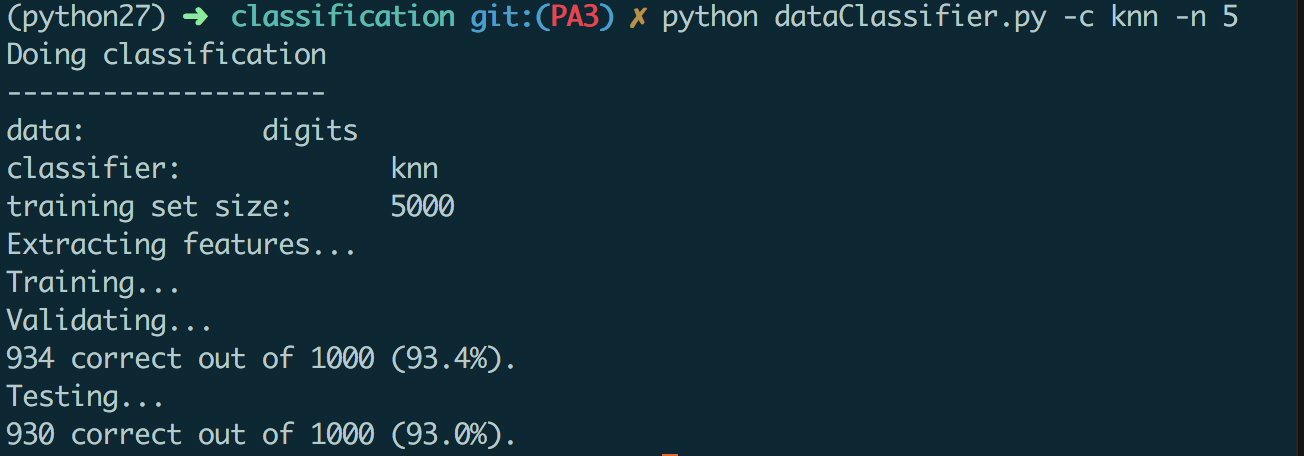
\includegraphics[width=6cm]{q_1.png}
		\caption{KNN}
		\label{KNN}
		\end{minipage}
		\centering
		\begin{minipage}[t]{0.4\textwidth}
		\centering
		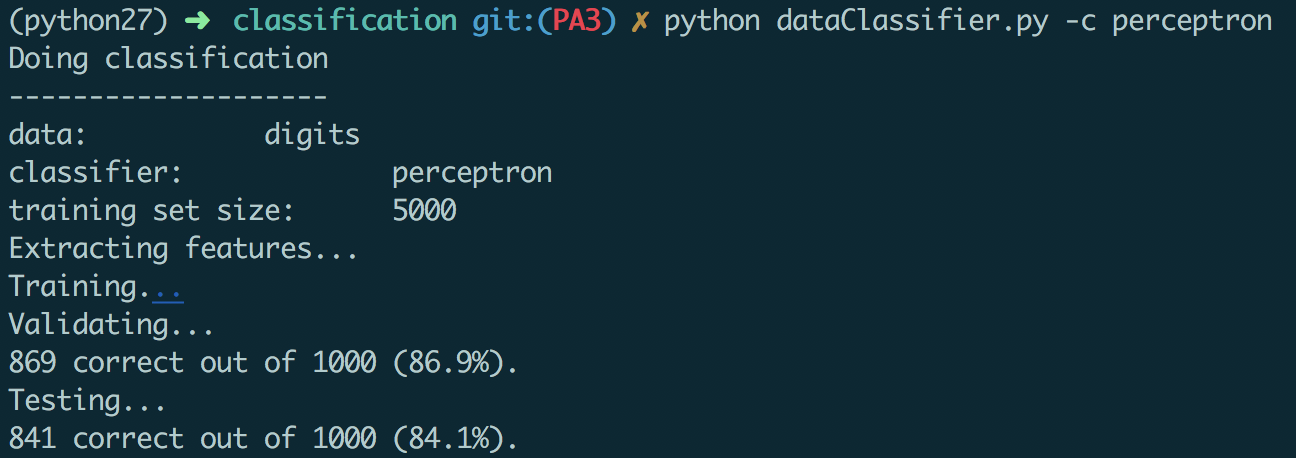
\includegraphics[width=6cm]{q_2.png}
		\caption{Perceptron}
		\label{Perceptron}
		\end{minipage}
		\centering
		\begin{minipage}[t]{0.4\textwidth}
		\centering
		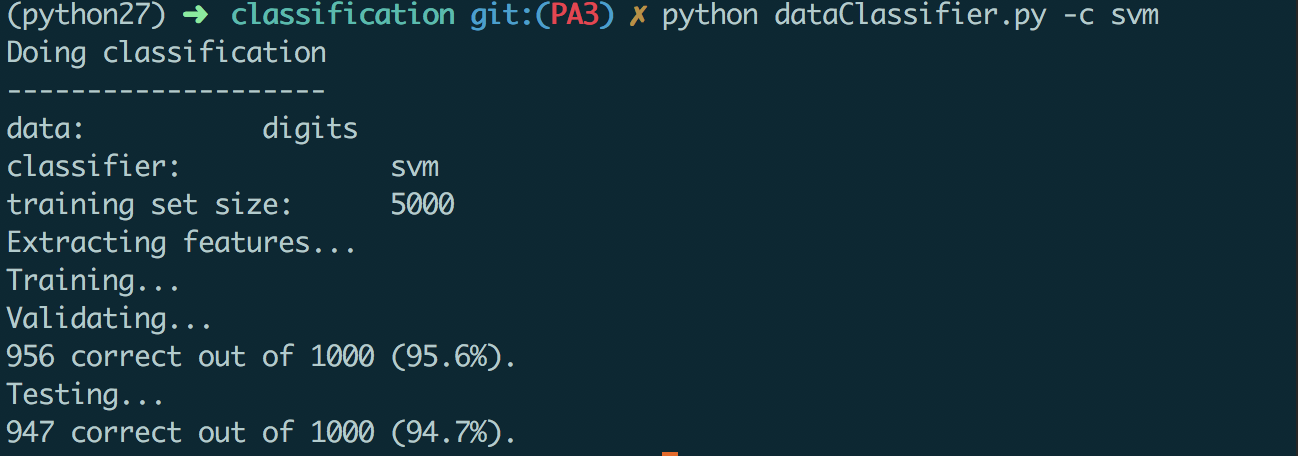
\includegraphics[width=6cm]{q_3.png}
		\caption{SVM with sklearn}
		\label{SVM}
		\end{minipage}
		\begin{minipage}[t]{0.4\textwidth}
		\centering
		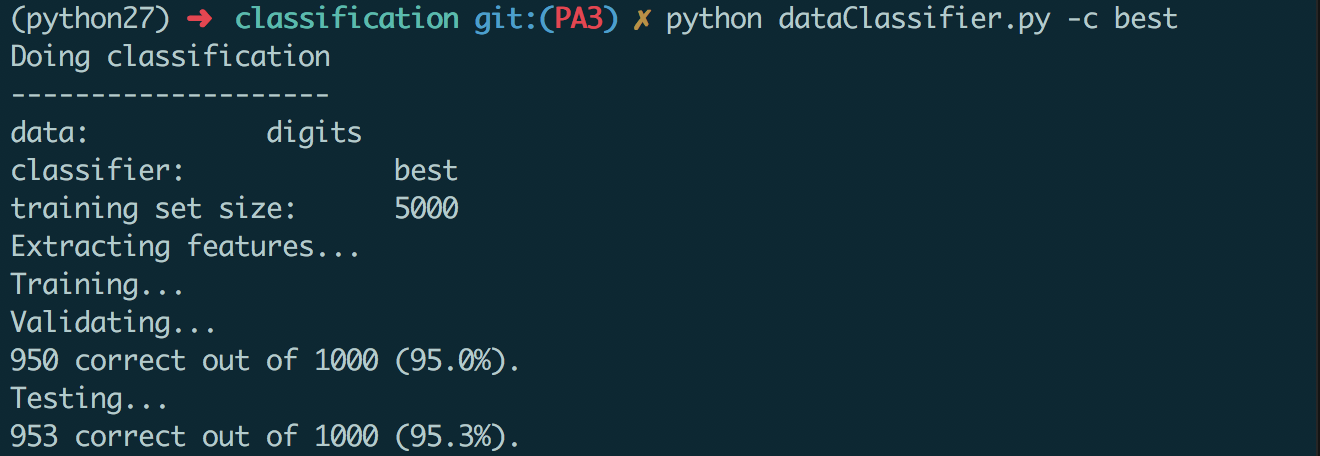
\includegraphics[width=6cm]{q_4.png}
		\caption{Better Classification Accuracy}
		\label{Better Classification Accuracy}
		\end{minipage}
	\end{figure}
	\paragraph{}
	Description: Implement a perception (or it can also be called softmax regression) classifier.
	\paragraph{}
	这一问中需要实现一个感知机,感知机需要通过在迭代过程中不断更新权重使得权重更能近似描述各种分类的特征,实现思路为:对每一个训练样本进行描述之后使用该训练样本的各个点的大小来更新权重,由于样本都是0-1之间的小数,所以使用这种方式最终结果大致为所有的同一类的样本进行叠加的效果,可以很好的描述各个分类。算法的测试结果如图\ref{Perceptron}。
	\paragraph{}
	这一问中需要对权重可视化的结果进行选择,由于感知机的权重需要用来描述每个分类下的所有特征,大致上为该分类下所有样本的叠加的效果,因此图像描述不可能为精准的图像,因此选择(a)选项。
	
\end{homeworkProblem}

\begin{homeworkProblem}[SVM with sklearn]
	
	\paragraph{}
	Description: Utilize the SVM algorithm in sklearn for classification.
	\paragraph{}
	这一问需要使用scikit-learn中的SVM的API进行实现,在进行一系列参数的设定之后,这一问的测试结果如图\ref{SVM}。使用的参数为$C=10, kernel = 'rbf'$。
	\paragraph{SVM的参数设定}
	SVM的参数如\ref{q_3}。其中$C$为惩罚参数,$C$越大,相当于惩罚松弛变量,希望松弛变量接近0,即对误分类的惩罚增大,趋向于对训练集全分对的情况,这样对训练集测试时准确率很高,但泛化能力弱。$C$值小,对误分类的惩罚减小,允许容错,将他们当成噪声点,泛化能力较强。$kernel$是核函数,默认是$rbf$,可以是$linear$, $poly$, $rbf$, $sigmoid$, $precomputed$ ,核函数主要用来针对线性不可分的情况,可以将数据映射到高维空间中来实现分割,在这个问题中,使用$rbf$有着较好的效果。$gamma$是$rbf$,$poly$和$sigmoid$的核函数参数。默认是$auto$,$gammma = \frac{1}{n\_features}$。
	\pythonscript{q_3}{SVM}
	\begin{figure}[ht]
		\centering
		\begin{minipage}[t]{0.4\textwidth}
		\centering
		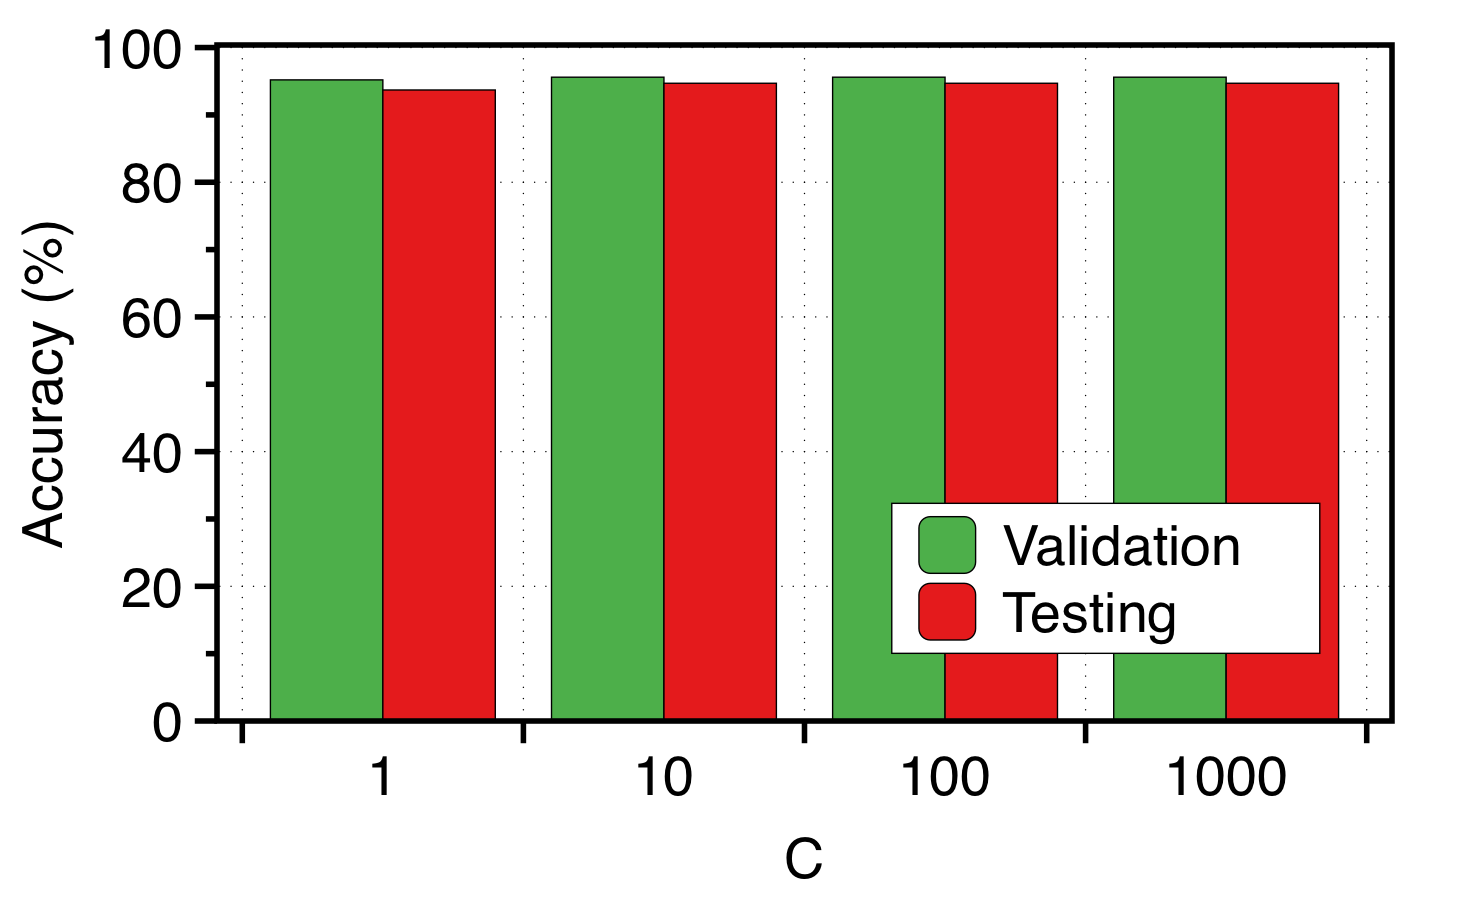
\includegraphics[width=6cm]{C.png}
		\caption{改变C值对准确率的影响}
		\label{C}
		\end{minipage}
		\centering
		\begin{minipage}[t]{0.4\textwidth}
		\centering
		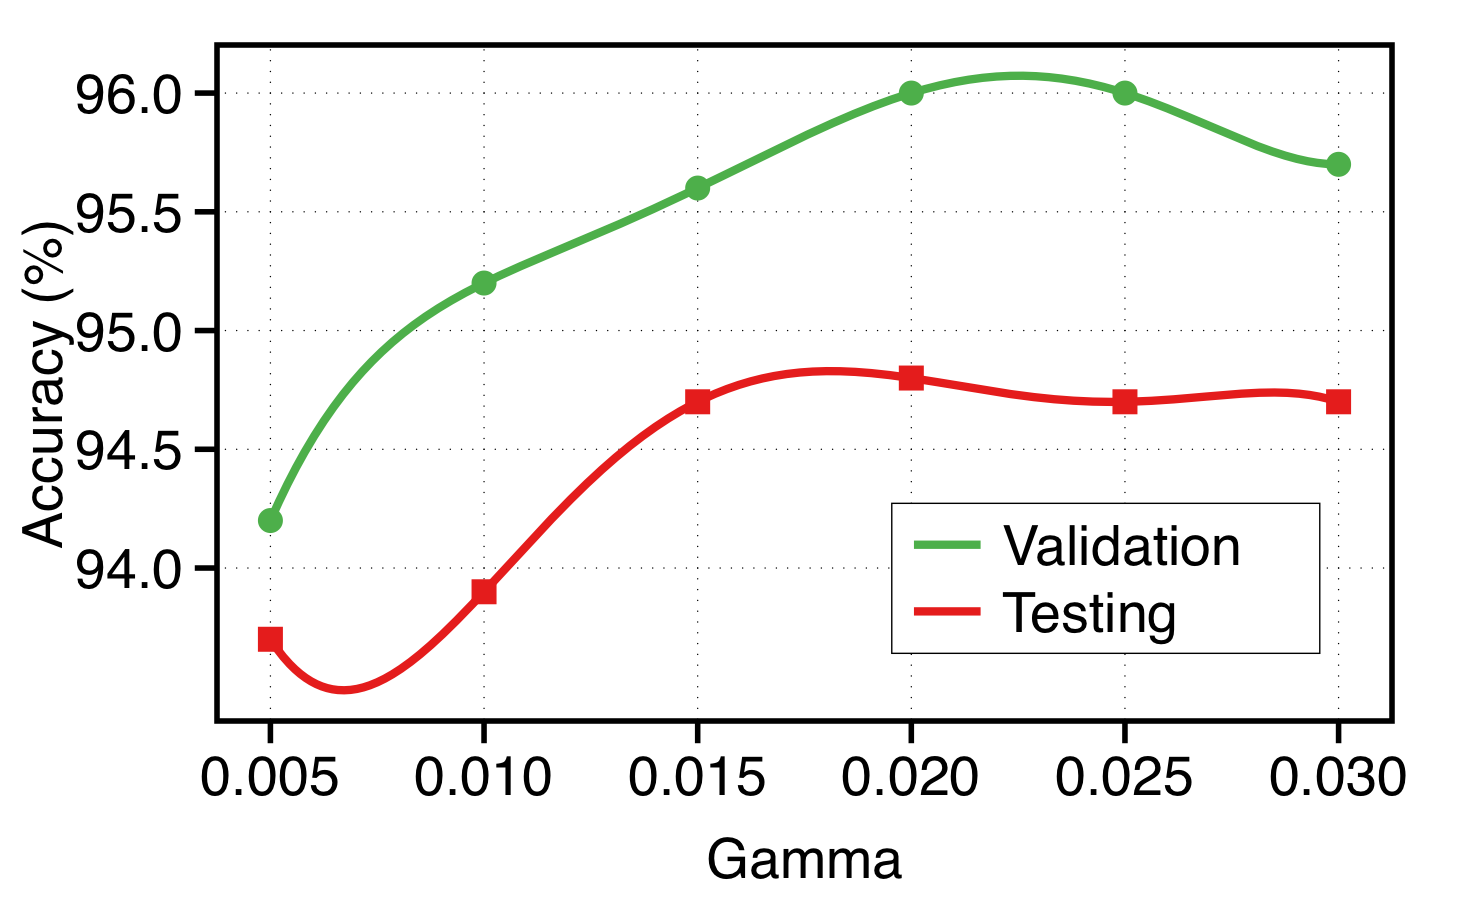
\includegraphics[width=6cm]{gamma.png}
		\caption{改变Gamma对准确率的影响}
		\label{gamma}
		\end{minipage}
		\centering
	\end{figure}
	\paragraph{SVM参数设定比较}
	改变SVM参数设定中的C值,预测函数的准确率会发生改变,在$gamma = 0.015$的情况下,设定$C$值分别为$1, 10, 100, 1000$对准确率进行测试,测试结果如图\ref{C}。可以看出,$C$值增大,准确率首先提高,但是当$C$值超出一定数值之后,其增大效果不再在准确率上体现出来,当$C = 1000$时,模型仍然没有表现出过拟合现象。之后,固定$C = 10$,对$Gamma$值进行改变,测试预测准确率如图\ref{gamma},可以看出,准确率对$Gamma$值的改变相对来说比较敏感,因此选择测试样本准确率最高的一组$gamma = 0.015$作为最终的参数。
\end{homeworkProblem}

\begin{homeworkProblem}[Better Classification Accuracy]
	\paragraph{}
	Description: Design a classification algorithm to get as best accuracy as you can.
	\paragraph{}
	这一问要求设计一个分类器,来实现良好的分类准确性,根据之前的分类效果来看,SVM具有较好的分类效果,因此这一问中继续采用scikit-learn的SVM作为分类器,主要目标是通过对超参数的调节实现较好的分类效果。
	\paragraph{}
	如果直接使用原始数据进行SVM分类,效果较差,因此考虑使用PCA进行特征提取降维,对降维之后的数据采用支持向量机进行分类。需要进行调整的超参数主要有PCA提取的特征数目,以及SVM中的想过超参数,经过多次测试$n\_components = 35, C=3, gamma=1/35.0$时整个模型有着较好的预测效果,测试的结果如图\ref{Better Classification Accuracy},模型在测试集上的准确率为$95.8\%$。
	\paragraph{}
	对于SVM的参数设定,如果设定的$C$值过大,那么模型对误分类的惩罚值过大,容易出现过拟合的现象,模型在验证集和测试集上的表现会很差。但是如果设定的值过小,则会出现特征不明确的现象,误分类比例较大,同样会造成表现差的现象。对于PCA提取特征数目的设定,如果设定的数目过低,那么提取出的特征无法准确描述该分类的特征,但是如果提取的数目过多,那么会造成对噪音的过滤不够完全,优化效果不够明显的现象。从最终测试得到的较优的参数设定以及测试结果来看,每个分类大致需要35个特征值就可以准确唯一描述,同时测试得到$C=100$的惩罚值设定并没有造成过拟合现象。
\end{homeworkProblem}

\end{document}